\documentclass[a4paper,10pt]{article}
\usepackage[breakable]{tcolorbox}
\usepackage{parskip} % Stop auto-indenting (to mimic markdown behaviour)

% Basic figure setup, for now with no caption control since it's done
% automatically by Pandoc (which extracts ![](path) syntax from Markdown).
\usepackage{graphicx}
% Maintain compatibility with old templates. Remove in nbconvert 6.0
% \let\Oldincludegraphics\includegraphics
% Ensure that by default, figures have no caption (until we provide a
% proper Figure object with a Caption API and a way to capture that
% in the conversion process - todo).
\usepackage{caption}
% \DeclareCaptionFormat{nocaption}{}
% \captionsetup{format=nocaption,aboveskip=0pt,belowskip=0pt}
\usepackage{float}
\floatplacement{figure}{H} % forces figures to be placed at the correct location
\usepackage{xcolor} % Allow colors to be defined
\usepackage{enumerate} % Needed for markdown enumerations to work
\usepackage{geometry} % Used to adjust the document margins
\usepackage{amsmath} % Equations
\usepackage{amssymb} % Equations
\usepackage{textcomp} % defines textquotesingle
% Hack from http://tex.stackexchange.com/a/47451/13684:
\AtBeginDocument{%
    \def\PYZsq{\textquotesingle}% Upright quotes in Pygmentized code
}
\usepackage{upquote} % Upright quotes for verbatim code
\usepackage{eurosym} % defines \euro
\usepackage{iftex}
\ifPDFTeX
    \usepackage[T1]{fontenc}
    \IfFileExists{alphabeta.sty}{
          \usepackage{alphabeta}
      }{
          \usepackage[mathletters]{ucs}
          \usepackage[utf8x]{inputenc}
      }
\else
    \usepackage{fontspec}
    \usepackage{unicode-math}
\fi
\usepackage{fancyvrb} % verbatim replacement that allows latex
\usepackage{grffile} % extends the file name processing of package graphics
                     % to support a larger range
\makeatletter % fix for old versions of grffile with XeLaTeX
\@ifpackagelater{grffile}{2019/11/01}
{
  % Do nothing on new versions
}
{
  \def\Gread@@xetex#1{%
    \IfFileExists{"\Gin@base".bb}%
    {\Gread@eps{\Gin@base.bb}}%
    {\Gread@@xetex@aux#1}%
  }
}
\makeatother
\usepackage[Export]{adjustbox} % Used to constrain images to a maximum size
\adjustboxset{max size={0.9\linewidth}{0.9\paperheight}}
% The hyperref package gives us a pdf with properly built
% internal navigation ('pdf bookmarks' for the table of contents,
% internal cross-reference links, web links for URLs, etc.)
\usepackage{hyperref}
% The default LaTeX title has an obnoxious amount of whitespace. By default,
% titling removes some of it. It also provides customization options.
\usepackage{titling}
\usepackage{longtable} % longtable support required by pandoc >1.10
\usepackage{booktabs}  % table support for pandoc > 1.12.2
\usepackage{array}     % table support for pandoc >= 2.11.3
\usepackage{calc}      % table minipage width calculation for pandoc >= 2.11.1
\usepackage[inline]{enumitem} % IRkernel/repr support (it uses the enumerate* environment)
\usepackage[normalem]{ulem} % ulem is needed to support strikethroughs (\sout)
                            % normalem makes italics be italics, not underlines
\usepackage{soul}      % strikethrough (\st) support for pandoc >= 3.0.0
\usepackage{mathrsfs}

\DeclareSymbolFont{symbols}{OMS}{cmsy}{m}{n}
\DeclareMathSymbol{\alpha}{\mathalpha}{symbols}{"0B}
\DeclareMathSymbol{\beta}{\mathalpha}{symbols}{"0C}
\DeclareMathSymbol{\gamma}{\mathalpha}{symbols}{"0D}
\DeclareMathSymbol{\delta}{\mathalpha}{symbols}{"0E}
\DeclareMathSymbol{\epsilon}{\mathalpha}{symbols}{"0F}
\DeclareMathSymbol{\zeta}{\mathalpha}{symbols}{"10}
\DeclareMathSymbol{\eta}{\mathalpha}{symbols}{"11}
\DeclareMathSymbol{\theta}{\mathalpha}{symbols}{"12}
\DeclareMathSymbol{\iota}{\mathalpha}{symbols}{"13}
\DeclareMathSymbol{\kappa}{\mathalpha}{symbols}{"14}
\DeclareMathSymbol{\lambda}{\mathalpha}{symbols}{"15}
\DeclareMathSymbol{\mu}{\mathalpha}{symbols}{"16}
\DeclareMathSymbol{\nu}{\mathalpha}{symbols}{"17}
\DeclareMathSymbol{\xi}{\mathalpha}{symbols}{"18}
\DeclareMathSymbol{\pi}{\mathalpha}{symbols}{"19}
\DeclareMathSymbol{\rho}{\mathalpha}{symbols}{"1A}
\DeclareMathSymbol{\sigma}{\mathalpha}{symbols}{"1B}
\DeclareMathSymbol{\tau}{\mathalpha}{symbols}{"1C}
\DeclareMathSymbol{\upsilon}{\mathalpha}{symbols}{"1D}
\DeclareMathSymbol{\phi}{\mathalpha}{symbols}{"1E}
\DeclareMathSymbol{\chi}{\mathalpha}{symbols}{"1F}
\DeclareMathSymbol{\psi}{\mathalpha}{symbols}{"20}
\DeclareMathSymbol{\omega}{\mathalpha}{symbols}{"21}

\usepackage{algorithm,algpseudocode,multirow}
\usepackage{lipsum}

\usepackage{fontawesome5}
\newcommand{\email}[1]{\faEnvelope\ {#1}}

\usepackage{enumitem}

% Colors for the hyperref package
% \definecolor{urlcolor}{rgb}{0,.145,.698}
% \definecolor{linkcolor}{rgb}{.71,0.21,0.01}
% \definecolor{citecolor}{rgb}{.12,.54,.11}
% ANSI colors
\definecolor{ansi-black}{HTML}{3E424D}
\definecolor{ansi-black-intense}{HTML}{282C36}
\definecolor{ansi-red}{HTML}{E75C58}
\definecolor{ansi-red-intense}{HTML}{B22B31}
\definecolor{ansi-green}{HTML}{00A250}
\definecolor{ansi-green-intense}{HTML}{007427}
\definecolor{ansi-yellow}{HTML}{DDB62B}
\definecolor{ansi-yellow-intense}{HTML}{B27D12}
\definecolor{ansi-blue}{HTML}{208FFB}
\definecolor{ansi-blue-intense}{HTML}{0065CA}
\definecolor{ansi-magenta}{HTML}{D160C4}
\definecolor{ansi-magenta-intense}{HTML}{A03196}
\definecolor{ansi-cyan}{HTML}{60C6C8}
\definecolor{ansi-cyan-intense}{HTML}{258F8F}
\definecolor{ansi-white}{HTML}{C5C1B4}
\definecolor{ansi-white-intense}{HTML}{A1A6B2}
\definecolor{ansi-default-inverse-fg}{HTML}{FFFFFF}
\definecolor{ansi-default-inverse-bg}{HTML}{000000}
% common color for the border for error outputs.
\definecolor{outerrorbackground}{HTML}{FFDFDF}
% commands and environments needed by pandoc snippets
% extracted from the output of `pandoc -s`
\providecommand{\tightlist}{%
  \setlength{\itemsep}{0pt}\setlength{\parskip}{0pt}}
\DefineVerbatimEnvironment{Highlighting}{Verbatim}{commandchars=\\\{\}}
% Add ',fontsize=\small' for more characters per line
\newenvironment{Shaded}{}{}
\newcommand{\KeywordTok}[1]{\textcolor[rgb]{0.00,0.44,0.13}{\textbf{{#1}}}}
\newcommand{\DataTypeTok}[1]{\textcolor[rgb]{0.56,0.13,0.00}{{#1}}}
\newcommand{\DecValTok}[1]{\textcolor[rgb]{0.25,0.63,0.44}{{#1}}}
\newcommand{\BaseNTok}[1]{\textcolor[rgb]{0.25,0.63,0.44}{{#1}}}
\newcommand{\FloatTok}[1]{\textcolor[rgb]{0.25,0.63,0.44}{{#1}}}
\newcommand{\CharTok}[1]{\textcolor[rgb]{0.25,0.44,0.63}{{#1}}}
\newcommand{\StringTok}[1]{\textcolor[rgb]{0.25,0.44,0.63}{{#1}}}
\newcommand{\CommentTok}[1]{\textcolor[rgb]{0.38,0.63,0.69}{\textit{{#1}}}}
\newcommand{\OtherTok}[1]{\textcolor[rgb]{0.00,0.44,0.13}{{#1}}}
\newcommand{\AlertTok}[1]{\textcolor[rgb]{1.00,0.00,0.00}{\textbf{{#1}}}}
\newcommand{\FunctionTok}[1]{\textcolor[rgb]{0.02,0.16,0.49}{{#1}}}
\newcommand{\RegionMarkerTok}[1]{{#1}}
\newcommand{\ErrorTok}[1]{\textcolor[rgb]{1.00,0.00,0.00}{\textbf{{#1}}}}
\newcommand{\NormalTok}[1]{{#1}}
% Additional commands for more recent versions of Pandoc
\newcommand{\ConstantTok}[1]{\textcolor[rgb]{0.53,0.00,0.00}{{#1}}}
\newcommand{\SpecialCharTok}[1]{\textcolor[rgb]{0.25,0.44,0.63}{{#1}}}
\newcommand{\VerbatimStringTok}[1]{\textcolor[rgb]{0.25,0.44,0.63}{{#1}}}
\newcommand{\SpecialStringTok}[1]{\textcolor[rgb]{0.73,0.40,0.53}{{#1}}}
\newcommand{\ImportTok}[1]{{#1}}
\newcommand{\DocumentationTok}[1]{\textcolor[rgb]{0.73,0.13,0.13}{\textit{{#1}}}}
\newcommand{\AnnotationTok}[1]{\textcolor[rgb]{0.38,0.63,0.69}{\textbf{\textit{{#1}}}}}
\newcommand{\CommentVarTok}[1]{\textcolor[rgb]{0.38,0.63,0.69}{\textbf{\textit{{#1}}}}}
\newcommand{\VariableTok}[1]{\textcolor[rgb]{0.10,0.09,0.49}{{#1}}}
\newcommand{\ControlFlowTok}[1]{\textcolor[rgb]{0.00,0.44,0.13}{\textbf{{#1}}}}
\newcommand{\OperatorTok}[1]{\textcolor[rgb]{0.40,0.40,0.40}{{#1}}}
\newcommand{\BuiltInTok}[1]{{#1}}
\newcommand{\ExtensionTok}[1]{{#1}}
\newcommand{\PreprocessorTok}[1]{\textcolor[rgb]{0.74,0.48,0.00}{{#1}}}
\newcommand{\AttributeTok}[1]{\textcolor[rgb]{0.49,0.56,0.16}{{#1}}}
\newcommand{\InformationTok}[1]{\textcolor[rgb]{0.38,0.63,0.69}{\textbf{\textit{{#1}}}}}
\newcommand{\WarningTok}[1]{\textcolor[rgb]{0.38,0.63,0.69}{\textbf{\textit{{#1}}}}}
% Define a nice break command that doesn't care if a line doesn't already
% exist.
\def\br{\hspace*{\fill} \\* }
% Math Jax compatibility definitions
\def\gt{>}
\def\lt{<}
\let\Oldtex\TeX
\let\Oldlatex\LaTeX
\renewcommand{\TeX}{\textrm{\Oldtex}}
\renewcommand{\LaTeX}{\textrm{\Oldlatex}}
% Document parameters

% Document title
\title{\huge
$\texttt{Meep}$ and $\texttt{MPB}$ in Computational Photonics \\
\vspace{0.5cm}
\rule{\linewidth}{0.1mm} \\
\vspace{2.0cm}
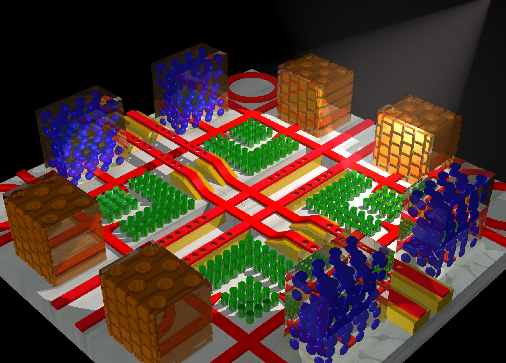
\includegraphics[scale=1.35]{photonic_micropolis_logo.pdf} \\
\vspace{1.5cm}
\small Figure downloaded from \url{http://ab-initio.mit.edu/photons/micropolis-hires.jpg} \\
\vspace{2.0cm}
\LARGE Ang Chen\bigskip}

\author{\color{magenta}\email{\href{mailto:chenang@outlook.com}{\LARGE\texttt{chenang@outlook.com}}}\\ 
\medskip}
\date{\LARGE\today}
% \date{November 8, 2023}

    
% Pygments definitions
\makeatletter
\def\PY@reset{\let\PY@it=\relax \let\PY@bf=\relax%
    \let\PY@ul=\relax \let\PY@tc=\relax%
    \let\PY@bc=\relax \let\PY@ff=\relax}
\def\PY@tok#1{\csname PY@tok@#1\endcsname}
\def\PY@toks#1+{\ifx\relax#1\empty\else%
    \PY@tok{#1}\expandafter\PY@toks\fi}
\def\PY@do#1{\PY@bc{\PY@tc{\PY@ul{%
    \PY@it{\PY@bf{\PY@ff{#1}}}}}}}
\def\PY#1#2{\PY@reset\PY@toks#1+\relax+\PY@do{#2}}

\@namedef{PY@tok@w}{\def\PY@tc##1{\textcolor[rgb]{0.73,0.73,0.73}{##1}}}
\@namedef{PY@tok@c}{\let\PY@it=\textit\def\PY@tc##1{\textcolor[rgb]{0.24,0.48,0.48}{##1}}}
\@namedef{PY@tok@cp}{\def\PY@tc##1{\textcolor[rgb]{0.61,0.40,0.00}{##1}}}
\@namedef{PY@tok@k}{\let\PY@bf=\textbf\def\PY@tc##1{\textcolor[rgb]{0.00,0.50,0.00}{##1}}}
\@namedef{PY@tok@kp}{\def\PY@tc##1{\textcolor[rgb]{0.00,0.50,0.00}{##1}}}
\@namedef{PY@tok@kt}{\def\PY@tc##1{\textcolor[rgb]{0.69,0.00,0.25}{##1}}}
\@namedef{PY@tok@o}{\def\PY@tc##1{\textcolor[rgb]{0.40,0.40,0.40}{##1}}}
\@namedef{PY@tok@ow}{\let\PY@bf=\textbf\def\PY@tc##1{\textcolor[rgb]{0.67,0.13,1.00}{##1}}}
\@namedef{PY@tok@nb}{\def\PY@tc##1{\textcolor[rgb]{0.00,0.50,0.00}{##1}}}
\@namedef{PY@tok@nf}{\def\PY@tc##1{\textcolor[rgb]{0.00,0.00,1.00}{##1}}}
\@namedef{PY@tok@nc}{\let\PY@bf=\textbf\def\PY@tc##1{\textcolor[rgb]{0.00,0.00,1.00}{##1}}}
\@namedef{PY@tok@nn}{\let\PY@bf=\textbf\def\PY@tc##1{\textcolor[rgb]{0.00,0.00,1.00}{##1}}}
\@namedef{PY@tok@ne}{\let\PY@bf=\textbf\def\PY@tc##1{\textcolor[rgb]{0.80,0.25,0.22}{##1}}}
\@namedef{PY@tok@nv}{\def\PY@tc##1{\textcolor[rgb]{0.10,0.09,0.49}{##1}}}
\@namedef{PY@tok@no}{\def\PY@tc##1{\textcolor[rgb]{0.53,0.00,0.00}{##1}}}
\@namedef{PY@tok@nl}{\def\PY@tc##1{\textcolor[rgb]{0.46,0.46,0.00}{##1}}}
\@namedef{PY@tok@ni}{\let\PY@bf=\textbf\def\PY@tc##1{\textcolor[rgb]{0.44,0.44,0.44}{##1}}}
\@namedef{PY@tok@na}{\def\PY@tc##1{\textcolor[rgb]{0.41,0.47,0.13}{##1}}}
\@namedef{PY@tok@nt}{\let\PY@bf=\textbf\def\PY@tc##1{\textcolor[rgb]{0.00,0.50,0.00}{##1}}}
\@namedef{PY@tok@nd}{\def\PY@tc##1{\textcolor[rgb]{0.67,0.13,1.00}{##1}}}
\@namedef{PY@tok@s}{\def\PY@tc##1{\textcolor[rgb]{0.73,0.13,0.13}{##1}}}
\@namedef{PY@tok@sd}{\let\PY@it=\textit\def\PY@tc##1{\textcolor[rgb]{0.73,0.13,0.13}{##1}}}
\@namedef{PY@tok@si}{\let\PY@bf=\textbf\def\PY@tc##1{\textcolor[rgb]{0.64,0.35,0.47}{##1}}}
\@namedef{PY@tok@se}{\let\PY@bf=\textbf\def\PY@tc##1{\textcolor[rgb]{0.67,0.36,0.12}{##1}}}
\@namedef{PY@tok@sr}{\def\PY@tc##1{\textcolor[rgb]{0.64,0.35,0.47}{##1}}}
\@namedef{PY@tok@ss}{\def\PY@tc##1{\textcolor[rgb]{0.10,0.09,0.49}{##1}}}
\@namedef{PY@tok@sx}{\def\PY@tc##1{\textcolor[rgb]{0.00,0.50,0.00}{##1}}}
\@namedef{PY@tok@m}{\def\PY@tc##1{\textcolor[rgb]{0.40,0.40,0.40}{##1}}}
\@namedef{PY@tok@gh}{\let\PY@bf=\textbf\def\PY@tc##1{\textcolor[rgb]{0.00,0.00,0.50}{##1}}}
\@namedef{PY@tok@gu}{\let\PY@bf=\textbf\def\PY@tc##1{\textcolor[rgb]{0.50,0.00,0.50}{##1}}}
\@namedef{PY@tok@gd}{\def\PY@tc##1{\textcolor[rgb]{0.63,0.00,0.00}{##1}}}
\@namedef{PY@tok@gi}{\def\PY@tc##1{\textcolor[rgb]{0.00,0.52,0.00}{##1}}}
\@namedef{PY@tok@gr}{\def\PY@tc##1{\textcolor[rgb]{0.89,0.00,0.00}{##1}}}
\@namedef{PY@tok@ge}{\let\PY@it=\textit}
\@namedef{PY@tok@gs}{\let\PY@bf=\textbf}
\@namedef{PY@tok@ges}{\let\PY@bf=\textbf\let\PY@it=\textit}
\@namedef{PY@tok@gp}{\let\PY@bf=\textbf\def\PY@tc##1{\textcolor[rgb]{0.00,0.00,0.50}{##1}}}
\@namedef{PY@tok@go}{\def\PY@tc##1{\textcolor[rgb]{0.44,0.44,0.44}{##1}}}
\@namedef{PY@tok@gt}{\def\PY@tc##1{\textcolor[rgb]{0.00,0.27,0.87}{##1}}}
\@namedef{PY@tok@err}{\def\PY@bc##1{{\setlength{\fboxsep}{\string -\fboxrule}\fcolorbox[rgb]{1.00,0.00,0.00}{1,1,1}{\strut ##1}}}}
\@namedef{PY@tok@kc}{\let\PY@bf=\textbf\def\PY@tc##1{\textcolor[rgb]{0.00,0.50,0.00}{##1}}}
\@namedef{PY@tok@kd}{\let\PY@bf=\textbf\def\PY@tc##1{\textcolor[rgb]{0.00,0.50,0.00}{##1}}}
\@namedef{PY@tok@kn}{\let\PY@bf=\textbf\def\PY@tc##1{\textcolor[rgb]{0.00,0.50,0.00}{##1}}}
\@namedef{PY@tok@kr}{\let\PY@bf=\textbf\def\PY@tc##1{\textcolor[rgb]{0.00,0.50,0.00}{##1}}}
\@namedef{PY@tok@bp}{\def\PY@tc##1{\textcolor[rgb]{0.00,0.50,0.00}{##1}}}
\@namedef{PY@tok@fm}{\def\PY@tc##1{\textcolor[rgb]{0.00,0.00,1.00}{##1}}}
\@namedef{PY@tok@vc}{\def\PY@tc##1{\textcolor[rgb]{0.10,0.09,0.49}{##1}}}
\@namedef{PY@tok@vg}{\def\PY@tc##1{\textcolor[rgb]{0.10,0.09,0.49}{##1}}}
\@namedef{PY@tok@vi}{\def\PY@tc##1{\textcolor[rgb]{0.10,0.09,0.49}{##1}}}
\@namedef{PY@tok@vm}{\def\PY@tc##1{\textcolor[rgb]{0.10,0.09,0.49}{##1}}}
\@namedef{PY@tok@sa}{\def\PY@tc##1{\textcolor[rgb]{0.73,0.13,0.13}{##1}}}
\@namedef{PY@tok@sb}{\def\PY@tc##1{\textcolor[rgb]{0.73,0.13,0.13}{##1}}}
\@namedef{PY@tok@sc}{\def\PY@tc##1{\textcolor[rgb]{0.73,0.13,0.13}{##1}}}
\@namedef{PY@tok@dl}{\def\PY@tc##1{\textcolor[rgb]{0.73,0.13,0.13}{##1}}}
\@namedef{PY@tok@s2}{\def\PY@tc##1{\textcolor[rgb]{0.73,0.13,0.13}{##1}}}
\@namedef{PY@tok@sh}{\def\PY@tc##1{\textcolor[rgb]{0.73,0.13,0.13}{##1}}}
\@namedef{PY@tok@s1}{\def\PY@tc##1{\textcolor[rgb]{0.73,0.13,0.13}{##1}}}
\@namedef{PY@tok@mb}{\def\PY@tc##1{\textcolor[rgb]{0.40,0.40,0.40}{##1}}}
\@namedef{PY@tok@mf}{\def\PY@tc##1{\textcolor[rgb]{0.40,0.40,0.40}{##1}}}
\@namedef{PY@tok@mh}{\def\PY@tc##1{\textcolor[rgb]{0.40,0.40,0.40}{##1}}}
\@namedef{PY@tok@mi}{\def\PY@tc##1{\textcolor[rgb]{0.40,0.40,0.40}{##1}}}
\@namedef{PY@tok@il}{\def\PY@tc##1{\textcolor[rgb]{0.40,0.40,0.40}{##1}}}
\@namedef{PY@tok@mo}{\def\PY@tc##1{\textcolor[rgb]{0.40,0.40,0.40}{##1}}}
\@namedef{PY@tok@ch}{\let\PY@it=\textit\def\PY@tc##1{\textcolor[rgb]{0.24,0.48,0.48}{##1}}}
\@namedef{PY@tok@cm}{\let\PY@it=\textit\def\PY@tc##1{\textcolor[rgb]{0.24,0.48,0.48}{##1}}}
\@namedef{PY@tok@cpf}{\let\PY@it=\textit\def\PY@tc##1{\textcolor[rgb]{0.24,0.48,0.48}{##1}}}
\@namedef{PY@tok@c1}{\let\PY@it=\textit\def\PY@tc##1{\textcolor[rgb]{0.24,0.48,0.48}{##1}}}
\@namedef{PY@tok@cs}{\let\PY@it=\textit\def\PY@tc##1{\textcolor[rgb]{0.24,0.48,0.48}{##1}}}

\def\PYZbs{\char`\\}
\def\PYZus{\char`\_}
\def\PYZob{\char`\{}
\def\PYZcb{\char`\}}
\def\PYZca{\char`\^}
\def\PYZam{\char`\&}
\def\PYZlt{\char`\<}
\def\PYZgt{\char`\>}
\def\PYZsh{\char`\#}
\def\PYZpc{\char`\%}
\def\PYZdl{\char`\$}
\def\PYZhy{\char`\-}
\def\PYZsq{\char`\'}
\def\PYZdq{\char`\"}
\def\PYZti{\char`\~}
% for compatibility with earlier versions
\def\PYZat{@}
\def\PYZlb{[}
\def\PYZrb{]}
\makeatother


% For linebreaks inside Verbatim environment from package fancyvrb.
\makeatletter
\newbox\Wrappedcontinuationbox
\newbox\Wrappedvisiblespacebox
\newcommand*\Wrappedvisiblespace {\textcolor{red}{\textvisiblespace}}
\newcommand*\Wrappedcontinuationsymbol {\textcolor{red}{\llap{\tiny$\m@th\hookrightarrow$}}}
\newcommand*\Wrappedcontinuationindent {3ex }
\newcommand*\Wrappedafterbreak {\kern\Wrappedcontinuationindent\copy\Wrappedcontinuationbox}
% Take advantage of the already applied Pygments mark-up to insert
% potential linebreaks for TeX processing.
%        {, <, #, %, $, ' and ": go to next line.
%        _, }, ^, &, >, - and ~: stay at end of broken line.
% Use of \textquotesingle for straight quote.
\newcommand*\Wrappedbreaksatspecials {%
    \def\PYGZus{\discretionary{\char`\_}{\Wrappedafterbreak}{\char`\_}}%
    \def\PYGZob{\discretionary{}{\Wrappedafterbreak\char`\{}{\char`\{}}%
    \def\PYGZcb{\discretionary{\char`\}}{\Wrappedafterbreak}{\char`\}}}%
    \def\PYGZca{\discretionary{\char`\^}{\Wrappedafterbreak}{\char`\^}}%
    \def\PYGZam{\discretionary{\char`\&}{\Wrappedafterbreak}{\char`\&}}%
    \def\PYGZlt{\discretionary{}{\Wrappedafterbreak\char`\<}{\char`\<}}%
    \def\PYGZgt{\discretionary{\char`\>}{\Wrappedafterbreak}{\char`\>}}%
    \def\PYGZsh{\discretionary{}{\Wrappedafterbreak\char`\#}{\char`\#}}%
    \def\PYGZpc{\discretionary{}{\Wrappedafterbreak\char`\%}{\char`\%}}%
    \def\PYGZdl{\discretionary{}{\Wrappedafterbreak\char`\$}{\char`\$}}%
    \def\PYGZhy{\discretionary{\char`\-}{\Wrappedafterbreak}{\char`\-}}%
    \def\PYGZsq{\discretionary{}{\Wrappedafterbreak\textquotesingle}{\textquotesingle}}%
    \def\PYGZdq{\discretionary{}{\Wrappedafterbreak\char`\"}{\char`\"}}%
    \def\PYGZti{\discretionary{\char`\~}{\Wrappedafterbreak}{\char`\~}}%
}
% Some characters . , ; ? ! / are not pygmentized.
% This macro makes them "active" and they will insert potential linebreaks
\newcommand*\Wrappedbreaksatpunct {%
    \lccode`\~`\.\lowercase{\def~}{\discretionary{\hbox{\char`\.}}{\Wrappedafterbreak}{\hbox{\char`\.}}}%
    \lccode`\~`\,\lowercase{\def~}{\discretionary{\hbox{\char`\,}}{\Wrappedafterbreak}{\hbox{\char`\,}}}%
    \lccode`\~`\;\lowercase{\def~}{\discretionary{\hbox{\char`\;}}{\Wrappedafterbreak}{\hbox{\char`\;}}}%
    \lccode`\~`\:\lowercase{\def~}{\discretionary{\hbox{\char`\:}}{\Wrappedafterbreak}{\hbox{\char`\:}}}%
    \lccode`\~`\?\lowercase{\def~}{\discretionary{\hbox{\char`\?}}{\Wrappedafterbreak}{\hbox{\char`\?}}}%
    \lccode`\~`\!\lowercase{\def~}{\discretionary{\hbox{\char`\!}}{\Wrappedafterbreak}{\hbox{\char`\!}}}%
    \lccode`\~`\/\lowercase{\def~}{\discretionary{\hbox{\char`\/}}{\Wrappedafterbreak}{\hbox{\char`\/}}}%
    \catcode`\.\active
    \catcode`\,\active
    \catcode`\;\active
    \catcode`\:\active
    \catcode`\?\active
    \catcode`\!\active
    \catcode`\/\active
    \lccode`\~`\~
}
\makeatother
\let\OriginalVerbatim=\Verbatim
\makeatletter
\renewcommand{\Verbatim}[1][1]{%
    %\parskip\z@skip
    \sbox\Wrappedcontinuationbox {\Wrappedcontinuationsymbol}%
    \sbox\Wrappedvisiblespacebox {\FV@SetupFont\Wrappedvisiblespace}%
    \def\FancyVerbFormatLine ##1{\hsize\linewidth
        \vtop{\raggedright\hyphenpenalty\z@\exhyphenpenalty\z@
            \doublehyphendemerits\z@\finalhyphendemerits\z@
            \strut ##1\strut}%
    }%
    % If the linebreak is at a space, the latter will be displayed as visible
    % space at end of first line, and a continuation symbol starts next line.
    % Stretch/shrink are however usually zero for typewriter font.
    \def\FV@Space {%
        \nobreak\hskip\z@ plus\fontdimen3\font minus\fontdimen4\font
        \discretionary{\copy\Wrappedvisiblespacebox}{\Wrappedafterbreak}
        {\kern\fontdimen2\font}%
    }%
    % Allow breaks at special characters using \PYG... macros.
    \Wrappedbreaksatspecials
    % Breaks at punctuation characters . , ; ? ! and / need catcode=\active
    \OriginalVerbatim[#1,codes*=\Wrappedbreaksatpunct]%
}
\makeatother
% Exact colors from NB
\definecolor{incolor}{HTML}{303F9F}
\definecolor{outcolor}{HTML}{D84315}
\definecolor{cellborder}{HTML}{CFCFCF}
\definecolor{cellbackground}{HTML}{F7F7F7}
% prompt
\makeatletter
\newcommand{\boxspacing}{\kern\kvtcb@left@rule\kern\kvtcb@boxsep}
\makeatother
\newcommand{\prompt}[4]{
    {\ttfamily\llap{{\color{#2}#1[#3]:\hspace{3pt}#4}}\vspace{-\baselineskip}}
}

%

% Prevent overflowing lines due to hard-to-break entities
\sloppy
% Setup hyperref package
\hypersetup{
  breaklinks=true,  % so long urls are correctly broken across lines
  colorlinks=true,
  urlcolor=magenta,
  linkcolor=magenta,
  citecolor=blue,
  }
% Slightly bigger margins than the latex defaults

\geometry{top=2cm,bottom=2.5cm,left=3cm,right=3cm}

\makeatletter
\renewenvironment{abstract}{%
    \large % 设置 abstract 内容的字体大小
    \begin{center}%
        \bfseries \Large Abstract % 设置标题的字体大小和样式
        \vspace{-.5em}%
        \vspace{15pt}%
    \end{center}%
    \list{}{%
        \setlength{\leftmargin}{0mm}% 设置边距
        \setlength{\rightmargin}{\leftmargin}%
    }%
    \item\relax%
}{
    \endlist
}
\makeatother
    
%%%%%%%%%%%%%%%%%%%%%%%%%%%%%%%%%%%%%%%%%%%%%%%%%%%%%%%%%%%%%%%%%%%%%%%%%%%%%%%%%%%
%%%%%%%%%%%%%%%%%%%%%%%%%%%%%%%%%%%%%% Main text %%%%%%%%%%%%%%%%%%%%%%%%%%%%%%%%%%
%%%%%%%%%%%%%%%%%%%%%%%%%%%%%%%%%%%%%%%%%%%%%%%%%%%%%%%%%%%%%%%%%%%%%%%%%%%%%%%%%%%

\begin{document}
    
\maketitle
\thispagestyle{empty}
% \begin{abstract}
% \noindent \lipsum[1-5]
% \end{abstract}

\newpage
\pagenumbering{Roman} 
\tableofcontents
% \thispagestyle{empty}
% \renewcommand{\listfigurename}{Figures}
% \listoffigures

% \renewcommand{\listtablename}{Tables}
% \listoftables

% \renewcommand{\listalgorithmname}{Algorithms}
% \listofalgorithms


\newpage

%%%%%%%% Start: content to be replaced %%%%%%%%
\pagenumbering{arabic}

\section{Introduction}\label{introduction}

Here we show how to .

In a word, we can use various fitting methods to fit the spectra and get
the parameters of the nanophotonics structures.

Thus, the procedure of fitting can be divided into two key steps: 
\begin{itemize}[leftmargin=*]
\item Build the model of the spectra, which can be an expression, or an
electromagnetic (EM) solver, or even a neural network. 
\item Use the fittingmethod to find the best parameters of the model.
\end{itemize}

Besides, we can also use the method of library searching (the library
can be constructed by simulated data from the EM solver or the neural
network, or by experimental data) to find the best-fit model.

\section{Installation}\label{import-libraries}

\begin{tcolorbox}[breakable, size=fbox, boxrule=1pt, pad at break*=1mm,colback=cellbackground, colframe=cellborder]
\prompt{In}{incolor}{1}{\boxspacing}
\begin{Verbatim}[commandchars=\\\{\}]
\PY{k+kn}{from} \PY{n+nn}{ipywidgets} \PY{k+kn}{import} \PY{n}{interact}\PY{p}{,} \PY{n}{widgets}
\PY{k+kn}{import} \PY{n+nn}{matplotlib}\PY{n+nn}{.}\PY{n+nn}{pyplot} \PY{k}{as} \PY{n+nn}{plt}
\PY{k+kn}{import} \PY{n+nn}{numpy} \PY{k}{as} \PY{n+nn}{np}
\PY{k+kn}{from} \PY{n+nn}{scipy}\PY{n+nn}{.}\PY{n+nn}{interpolate} \PY{k+kn}{import} \PY{n}{interp1d}

\PY{n}{plt}\PY{o}{.}\PY{n}{rcParams}\PY{p}{[}\PY{l+s+s2}{\PYZdq{}}\PY{l+s+s2}{font.family}\PY{l+s+s2}{\PYZdq{}}\PY{p}{]} \PY{o}{=} \PY{l+s+s2}{\PYZdq{}}\PY{l+s+s2}{Helvetica}\PY{l+s+s2}{\PYZdq{}}
\PY{o}{\PYZpc{}}\PY{k}{matplotlib} inline
\PY{o}{\PYZpc{}}\PY{k}{config} InlineBackend.figure\PYZus{}format = \PYZsq{}svg\PYZsq{}
\end{Verbatim}
\end{tcolorbox}

\section{Tutorial}\label{formulation}

\subsection{Spectra of thin films}\label{spectra-of-thin-films}

First load the refractive index data of Si.

\begin{tcolorbox}[breakable, size=fbox, boxrule=1pt, pad at break*=1mm,colback=cellbackground, colframe=cellborder]
\prompt{In}{incolor}{2}{\boxspacing}
\begin{Verbatim}[commandchars=\\\{\}]
\PY{n}{data\PYZus{}Si} \PY{o}{=} \PY{n}{np}\PY{o}{.}\PY{n}{loadtxt}\PY{p}{(}\PY{l+s+s2}{\PYZdq{}}\PY{l+s+s2}{./data/Si.txt}\PY{l+s+s2}{\PYZdq{}}\PY{p}{,} \PY{n}{delimiter}\PY{o}{=}\PY{l+s+s1}{\PYZsq{}}\PY{l+s+se}{\PYZbs{}t}\PY{l+s+s1}{\PYZsq{}}\PY{p}{,} \PY{n}{skiprows}\PY{o}{=}\PY{l+m+mi}{1}\PY{p}{)}
\PY{n}{lda\PYZus{}Si} \PY{o}{=} \PY{n}{data\PYZus{}Si}\PY{p}{[}\PY{p}{:}\PY{p}{,} \PY{l+m+mi}{0}\PY{p}{]}
\PY{n}{n\PYZus{}Si} \PY{o}{=} \PY{n}{data\PYZus{}Si}\PY{p}{[}\PY{p}{:}\PY{p}{,} \PY{l+m+mi}{1}\PY{p}{]}
\PY{n}{k\PYZus{}Si} \PY{o}{=} \PY{n}{data\PYZus{}Si}\PY{p}{[}\PY{p}{:}\PY{p}{,} \PY{l+m+mi}{2}\PY{p}{]}

\PY{n}{n\PYZus{}Si\PYZus{}interp} \PY{o}{=} \PY{n}{interp1d}\PY{p}{(}\PY{n}{lda\PYZus{}Si}\PY{p}{,} \PY{n}{n\PYZus{}Si}\PY{p}{)}
\PY{n}{k\PYZus{}Si\PYZus{}interp} \PY{o}{=} \PY{n}{interp1d}\PY{p}{(}\PY{n}{lda\PYZus{}Si}\PY{p}{,} \PY{n}{k\PYZus{}Si}\PY{p}{)}
\end{Verbatim}
\end{tcolorbox}

Define the Cauchy model for Refractive index of SiO2.

\begin{tcolorbox}[breakable, size=fbox, boxrule=1pt, pad at break*=1mm,colback=cellbackground, colframe=cellborder]
\prompt{In}{incolor}{3}{\boxspacing}
\begin{Verbatim}[commandchars=\\\{\}]
\PY{k}{def} \PY{n+nf}{n\PYZus{}index\PYZus{}SiO2}\PY{p}{(}\PY{n}{A}\PY{p}{,} \PY{n}{B}\PY{p}{,} \PY{n}{lda}\PY{p}{)}\PY{p}{:}
    \PY{k}{return} \PY{n}{A} \PY{o}{+} \PY{n}{B}\PY{o}{/}\PY{n}{lda}\PY{o}{*}\PY{o}{*}\PY{l+m+mi}{2}
\end{Verbatim}
\end{tcolorbox}

Load the simulated spectrum.

\begin{tcolorbox}[breakable, size=fbox, boxrule=1pt, pad at break*=1mm,colback=cellbackground, colframe=cellborder]
\prompt{In}{incolor}{4}{\boxspacing}
\begin{Verbatim}[commandchars=\\\{\}]
\PY{n}{data\PYZus{}sim} \PY{o}{=} \PY{n}{np}\PY{o}{.}\PY{n}{loadtxt}\PY{p}{(}\PY{l+s+s1}{\PYZsq{}}\PY{l+s+s1}{./data/S4\PYZus{}Rp\PYZus{}SiO2onSi.csv}\PY{l+s+s1}{\PYZsq{}}\PY{p}{,} \PY{n}{delimiter}\PY{o}{=}\PY{l+s+s1}{\PYZsq{}}\PY{l+s+s1}{,}\PY{l+s+s1}{\PYZsq{}}\PY{p}{,} \PY{n}{skiprows}\PY{o}{=}\PY{l+m+mi}{1}\PY{p}{)}
\PY{n}{lda\PYZus{}array} \PY{o}{=} \PY{n}{data\PYZus{}sim}\PY{p}{[}\PY{p}{:}\PY{p}{,} \PY{l+m+mi}{0}\PY{p}{]}
\PY{n}{Rp\PYZus{}sim} \PY{o}{=} \PY{n}{data\PYZus{}sim}\PY{p}{[}\PY{p}{:}\PY{p}{,} \PY{l+m+mi}{1}\PY{p}{]}
\end{Verbatim}
\end{tcolorbox}

Next we define a function of fit the two curves: - Simulated spectrum -
Analytical spectrum

\begin{tcolorbox}[breakable, size=fbox, boxrule=1pt, pad at break*=1mm,colback=cellbackground, colframe=cellborder]
\prompt{In}{incolor}{5}{\boxspacing}
\begin{Verbatim}[commandchars=\\\{\}]
\PY{k}{def} \PY{n+nf}{fit\PYZus{}SiO2onSi}\PY{p}{(}\PY{n}{d\PYZus{}SiO2}\PY{p}{,} \PY{n}{A}\PY{p}{,} \PY{n}{B}\PY{p}{)}\PY{p}{:}
\PY{+w}{    }\PY{l+s+sd}{\PYZdq{}\PYZdq{}\PYZdq{}}
\PY{l+s+sd}{    Fit simulated curve and analytical curve.}

\PY{l+s+sd}{    Args:}
\PY{l+s+sd}{        d\PYZus{}SiO2 (float): Thickness of SiO2 layer (nm).}
\PY{l+s+sd}{        A (float): Parameter A in Cauchy model.}
\PY{l+s+sd}{        B (float): Parameter B in Cauchy model. (nm\PYZca{}2)}
\PY{l+s+sd}{    \PYZdq{}\PYZdq{}\PYZdq{}}
    \PY{n}{r\PYZus{}numerator} \PY{o}{=} \PY{n}{np}\PY{o}{.}\PY{n}{e} \PY{o}{*}\PY{o}{*} \PY{p}{(}
        \PY{l+m+mi}{4} \PY{o}{*} \PY{l+m+mi}{1}\PY{n}{j} \PY{o}{*} \PY{n}{d\PYZus{}SiO2} \PY{o}{*} \PY{n}{n\PYZus{}index\PYZus{}SiO2}\PY{p}{(}\PY{n}{A}\PY{p}{,} \PY{n}{B}\PY{p}{,} \PY{n}{lda\PYZus{}array}\PY{p}{)} \PY{o}{*} \PY{n}{np}\PY{o}{.}\PY{n}{pi} \PY{o}{/} \PY{n}{lda\PYZus{}array}
    \PY{p}{)} \PY{o}{*} \PY{p}{(}\PY{l+m+mi}{1} \PY{o}{+} \PY{n}{n\PYZus{}index\PYZus{}SiO2}\PY{p}{(}\PY{n}{A}\PY{p}{,} \PY{n}{B}\PY{p}{,} \PY{n}{lda\PYZus{}array}\PY{p}{)}\PY{p}{)} \PY{o}{*} \PY{p}{(}
        \PY{o}{\PYZhy{}}\PY{l+m+mi}{1}\PY{n}{j} \PY{o}{*} \PY{n}{k\PYZus{}Si\PYZus{}interp}\PY{p}{(}\PY{n}{lda\PYZus{}array}\PY{p}{)}
        \PY{o}{\PYZhy{}} \PY{n}{n\PYZus{}Si\PYZus{}interp}\PY{p}{(}\PY{n}{lda\PYZus{}array}\PY{p}{)}
        \PY{o}{+} \PY{n}{n\PYZus{}index\PYZus{}SiO2}\PY{p}{(}\PY{n}{A}\PY{p}{,} \PY{n}{B}\PY{p}{,} \PY{n}{lda\PYZus{}array}\PY{p}{)}
    \PY{p}{)} \PY{o}{\PYZhy{}} \PY{p}{(}\PY{o}{\PYZhy{}}\PY{l+m+mi}{1} \PY{o}{+} \PY{n}{n\PYZus{}index\PYZus{}SiO2}\PY{p}{(}\PY{n}{A}\PY{p}{,} \PY{n}{B}\PY{p}{,} \PY{n}{lda\PYZus{}array}\PY{p}{)}\PY{p}{)} \PY{o}{*} \PY{p}{(}
        \PY{l+m+mi}{1}\PY{n}{j} \PY{o}{*} \PY{n}{k\PYZus{}Si\PYZus{}interp}\PY{p}{(}\PY{n}{lda\PYZus{}array}\PY{p}{)}
        \PY{o}{+} \PY{n}{n\PYZus{}Si\PYZus{}interp}\PY{p}{(}\PY{n}{lda\PYZus{}array}\PY{p}{)}
        \PY{o}{+} \PY{n}{n\PYZus{}index\PYZus{}SiO2}\PY{p}{(}\PY{n}{A}\PY{p}{,} \PY{n}{B}\PY{p}{,} \PY{n}{lda\PYZus{}array}\PY{p}{)}
    \PY{p}{)}
    \PY{n}{r\PYZus{}denominator} \PY{o}{=} \PY{o}{\PYZhy{}}\PY{p}{(}
        \PY{n}{np}\PY{o}{.}\PY{n}{e} \PY{o}{*}\PY{o}{*} \PY{p}{(}\PY{l+m+mi}{4} \PY{o}{*} \PY{l+m+mi}{1}\PY{n}{j} \PY{o}{*} \PY{n}{d\PYZus{}SiO2} \PY{o}{*} \PY{n}{n\PYZus{}index\PYZus{}SiO2}\PY{p}{(}\PY{n}{A}\PY{p}{,} \PY{n}{B}\PY{p}{,} \PY{n}{lda\PYZus{}array}\PY{p}{)} \PY{o}{*} \PY{n}{np}\PY{o}{.}\PY{n}{pi} \PY{o}{/} \PY{n}{lda\PYZus{}array}\PY{p}{)}
    \PY{p}{)} \PY{o}{*} \PY{p}{(}\PY{o}{\PYZhy{}}\PY{l+m+mi}{1} \PY{o}{+} \PY{n}{n\PYZus{}index\PYZus{}SiO2}\PY{p}{(}\PY{n}{A}\PY{p}{,} \PY{n}{B}\PY{p}{,} \PY{n}{lda\PYZus{}array}\PY{p}{)}\PY{p}{)} \PY{o}{*} \PY{p}{(}
        \PY{o}{\PYZhy{}}\PY{l+m+mi}{1}\PY{n}{j} \PY{o}{*} \PY{n}{k\PYZus{}Si\PYZus{}interp}\PY{p}{(}\PY{n}{lda\PYZus{}array}\PY{p}{)}
        \PY{o}{\PYZhy{}} \PY{n}{n\PYZus{}Si\PYZus{}interp}\PY{p}{(}\PY{n}{lda\PYZus{}array}\PY{p}{)}
        \PY{o}{+} \PY{n}{n\PYZus{}index\PYZus{}SiO2}\PY{p}{(}\PY{n}{A}\PY{p}{,} \PY{n}{B}\PY{p}{,} \PY{n}{lda\PYZus{}array}\PY{p}{)}
    \PY{p}{)} \PY{o}{+} \PY{p}{(}\PY{l+m+mi}{1} \PY{o}{+} \PY{n}{n\PYZus{}index\PYZus{}SiO2}\PY{p}{(}\PY{n}{A}\PY{p}{,} \PY{n}{B}\PY{p}{,} \PY{n}{lda\PYZus{}array}\PY{p}{)}\PY{p}{)} \PY{o}{*} \PY{p}{(}
        \PY{l+m+mi}{1}\PY{n}{j} \PY{o}{*} \PY{n}{k\PYZus{}Si\PYZus{}interp}\PY{p}{(}\PY{n}{lda\PYZus{}array}\PY{p}{)}
        \PY{o}{+} \PY{n}{n\PYZus{}Si\PYZus{}interp}\PY{p}{(}\PY{n}{lda\PYZus{}array}\PY{p}{)}
        \PY{o}{+} \PY{n}{n\PYZus{}index\PYZus{}SiO2}\PY{p}{(}\PY{n}{A}\PY{p}{,} \PY{n}{B}\PY{p}{,} \PY{n}{lda\PYZus{}array}\PY{p}{)}
    \PY{p}{)}

    \PY{n}{Rp\PYZus{}ana} \PY{o}{=} \PY{n}{np}\PY{o}{.}\PY{n}{abs}\PY{p}{(}\PY{n}{r\PYZus{}numerator} \PY{o}{/} \PY{n}{r\PYZus{}denominator}\PY{p}{)} \PY{o}{*}\PY{o}{*} \PY{l+m+mi}{2}

    \PY{n}{fig}\PY{p}{,} \PY{n}{ax} \PY{o}{=} \PY{n}{plt}\PY{o}{.}\PY{n}{subplots}\PY{p}{(}\PY{l+m+mi}{1}\PY{p}{,} \PY{l+m+mi}{1}\PY{p}{,} \PY{n}{figsize}\PY{o}{=}\PY{p}{(}\PY{l+m+mi}{5}\PY{p}{,} \PY{l+m+mi}{3}\PY{p}{)}\PY{p}{)}
    \PY{n}{ax}\PY{o}{.}\PY{n}{plot}\PY{p}{(}\PY{n}{lda\PYZus{}array}\PY{p}{,} \PY{n}{Rp\PYZus{}sim}\PY{p}{,} \PY{n}{color}\PY{o}{=}\PY{l+s+s2}{\PYZdq{}}\PY{l+s+s2}{gray}\PY{l+s+s2}{\PYZdq{}}\PY{p}{,} \PY{n}{label}\PY{o}{=}\PY{l+s+s2}{\PYZdq{}}\PY{l+s+s2}{sim.}\PY{l+s+s2}{\PYZdq{}}\PY{p}{)}
    \PY{n}{ax}\PY{o}{.}\PY{n}{plot}\PY{p}{(}\PY{n}{lda\PYZus{}array}\PY{p}{,} \PY{n}{Rp\PYZus{}ana}\PY{p}{,} \PY{n}{color}\PY{o}{=}\PY{l+s+s2}{\PYZdq{}}\PY{l+s+s2}{blue}\PY{l+s+s2}{\PYZdq{}}\PY{p}{,} \PY{n}{lw}\PY{o}{=}\PY{l+m+mi}{1}\PY{p}{,} \PY{n}{label}\PY{o}{=}\PY{l+s+s2}{\PYZdq{}}\PY{l+s+s2}{fit.}\PY{l+s+s2}{\PYZdq{}}\PY{p}{)}
    \PY{n}{ax}\PY{o}{.}\PY{n}{set\PYZus{}xlabel}\PY{p}{(}\PY{l+s+s2}{\PYZdq{}}\PY{l+s+s2}{Wavelength (nm)}\PY{l+s+s2}{\PYZdq{}}\PY{p}{)}
    \PY{n}{ax}\PY{o}{.}\PY{n}{set\PYZus{}ylabel}\PY{p}{(}\PY{l+s+s2}{\PYZdq{}}\PY{l+s+s2}{Reflectivity}\PY{l+s+s2}{\PYZdq{}}\PY{p}{)}
    \PY{n}{ax}\PY{o}{.}\PY{n}{set\PYZus{}xlim}\PY{p}{(}\PY{p}{[}\PY{l+m+mi}{250}\PY{p}{,} \PY{l+m+mi}{850}\PY{p}{]}\PY{p}{)}
    \PY{n}{ax}\PY{o}{.}\PY{n}{set\PYZus{}ylim}\PY{p}{(}\PY{p}{[}\PY{l+m+mi}{0}\PY{p}{,} \PY{l+m+mi}{1}\PY{p}{]}\PY{p}{)}
    \PY{n}{ax}\PY{o}{.}\PY{n}{legend}\PY{p}{(}\PY{n}{loc}\PY{o}{=}\PY{l+m+mi}{1}\PY{p}{)}
    \PY{n}{fig}\PY{o}{.}\PY{n}{tight\PYZus{}layout}\PY{p}{(}\PY{p}{)}
\end{Verbatim}
\end{tcolorbox}

\begin{tcolorbox}[breakable, size=fbox, boxrule=1pt, pad at break*=1mm,colback=cellbackground, colframe=cellborder]
\prompt{In}{incolor}{6}{\boxspacing}
\begin{Verbatim}[commandchars=\\\{\}]
\PY{n}{interact}\PY{p}{(}
    \PY{n}{fit\PYZus{}SiO2onSi}\PY{p}{,}
    \PY{n}{d\PYZus{}SiO2}\PY{o}{=}\PY{n}{widgets}\PY{o}{.}\PY{n}{FloatSlider}\PY{p}{(}\PY{n}{value}\PY{o}{=}\PY{l+m+mi}{500}\PY{p}{,} \PY{n+nb}{min}\PY{o}{=}\PY{l+m+mi}{450}\PY{p}{,} \PY{n+nb}{max}\PY{o}{=}\PY{l+m+mi}{550}\PY{p}{,} \PY{n}{step}\PY{o}{=}\PY{l+m+mf}{0.1}\PY{p}{)}\PY{p}{,}
    \PY{n}{A}\PY{o}{=}\PY{n}{widgets}\PY{o}{.}\PY{n}{FloatSlider}\PY{p}{(}\PY{n}{valuse}\PY{o}{=}\PY{l+m+mf}{1.447}\PY{p}{,} \PY{n+nb}{min}\PY{o}{=}\PY{l+m+mf}{1.3}\PY{p}{,} \PY{n+nb}{max}\PY{o}{=}\PY{l+m+mf}{1.6}\PY{p}{,} \PY{n}{step}\PY{o}{=}\PY{l+m+mf}{0.001}\PY{p}{)}\PY{p}{,}
    \PY{n}{B}\PY{o}{=}\PY{n}{widgets}\PY{o}{.}\PY{n}{FloatSlider}\PY{p}{(}\PY{n}{value}\PY{o}{=}\PY{l+m+mi}{3540}\PY{p}{,} \PY{n+nb}{min}\PY{o}{=}\PY{l+m+mi}{3300}\PY{p}{,} \PY{n+nb}{max}\PY{o}{=}\PY{l+m+mi}{3600}\PY{p}{,} \PY{n}{step}\PY{o}{=}\PY{l+m+mi}{10}\PY{p}{)}\PY{p}{,}
\PY{p}{)}
\end{Verbatim}
\end{tcolorbox}

\begin{Verbatim}[commandchars=\\\{\}]
interactive(children=(FloatSlider(value=500.0, description='d\_SiO2', max=550.0, min=450.0), FloatSlider(value=…
\end{Verbatim}

    
\begin{tcolorbox}[breakable, size=fbox, boxrule=.5pt, pad at break*=1mm, opacityfill=0]
\prompt{Out}{outcolor}{6}{\boxspacing}
\begin{Verbatim}[commandchars=\\\{\}]
<function \_\_main\_\_.fit\_SiO2onSi(d\_SiO2, A, B)>
\end{Verbatim}
\end{tcolorbox}
        
\subsection{Spectra of photonic crystal
slabs}\label{spectra-of-photonic-crystal-slabs}

$\omega a/2\pi c$


%%%%%%%% End: content to be replaced %%%%%%%%
\newpage
\phantomsection
\addcontentsline{toc}{section}{References}
\begin{thebibliography}{99}

\bibitem{liu2012S4}
Victor Liu and Shanhui Fan.
\textit{S4: A free electromagnetic solver for layered periodic structures}.
Computer Physics Communications \textbf{183}: 2233, 2012.

\bibitem{li1997new}
Lifeng Li.
\textit{New formulation of the Fourier modal method for crossed surface-relief gratings}.
Journal of the Optical Society of America B \textbf{14}: 2758, 1997.

\bibitem{anderson1999LAPACK}
E. Anderson, Z. Bai, C. Bischof, S. Blackford, J. Demmel, J. Dongarra, J. Du Croz, A. Greenbaum, S. Hammarling, A. McKenney, D. Sorensen.
\textit{LAPACK Users' Guide}, 3rd ed.
(Society for Industrial and Applied Mathematics, Philadelphia, PA, 1999).

\end{thebibliography}

\end{document}
